% Created 2026-02-03 mar 20:14
% Intended LaTeX compiler: pdflatex
\documentclass[11pt, aspectratio=169, xcolor=table]{beamer}
\usepackage[utf8]{inputenc}
\usepackage[T1]{fontenc}
\usepackage{graphicx}
\usepackage{longtable}
\usepackage{wrapfig}
\usepackage{rotating}
\usepackage[normalem]{ulem}
\usepackage{amsmath}
\usepackage{amssymb}
\usepackage{capt-of}
\usepackage{hyperref}
\usepackage[spanish]{babel}
\usepackage[version=4]{mhchem}
\usepackage{ragged2e}
\renewcommand{\raggedright}{\justifying}
\usepackage{lmodern}
\usepackage{pdfrender}
\usepackage{tikz}
\usepackage{xcolor}
\usepackage{cite}
\usepackage{smartdiagram}
\usepackage{chemfig}
\usetheme{Berlin}
\author{Prof. Daniel Muñoz}
\date{\textit{<2025-03-06 jue>}}
\title{Química}
\subtitle{Unidad 1}
\titlegraphic{\includegraphics[width=4cm]{../img/udplogo}}
\hypersetup{
 pdfauthor={Prof. Daniel Muñoz},
 pdftitle={Química},
 pdfkeywords={},
 pdfsubject={},
 pdfcreator={Emacs 30.2 (Org mode 9.7.39)}, 
 pdflang={Spanish}}
\begin{document}

\maketitle
\begin{frame}{Outline}
\tableofcontents
\end{frame}

\section{Presentación}
\label{sec:org1363c2e}
\begin{frame}[label={sec:org888dd35}]{Acerca del Profesor}
\begin{columns}
\begin{column}{0.5\columnwidth}
\footnotesize
\begin{itemize}[<+->]
\item Daniel E. Muñoz Masson daniel.munoz3@mail.udp.cl
\item Profesor de Química. Uchile
\item Mg. en educación c/m Evaluación de Aprendizajes
\item Mg. En Ciencias Químicas c/m Fisicoquímica. Uchile
\item Analista Data Science con Python. Corfo
\item Analista QA en Automatización de Pruebas. Corfo
\item Experiencia como: Jefe de Proyectos, Docente, Automatizador, Académico-Investigador.
\end{itemize}
\end{column}
\begin{column}{0.5\columnwidth}
\begin{figure}[htbp]
\centering
\includegraphics[width=0.8\textwidth]{../img/yo.jpg}
\caption{\emph{Le Fils de l'Homme} 1964 René Magritte}
\end{figure}
\end{column}
\end{columns}
\end{frame}
\begin{frame}[label={sec:orgf0d75c9}]{Acerca del Curso}
\begin{columns}
\begin{column}{0.5\columnwidth}
\begin{itemize}
\item Horario: Mar y Jue 11:30 a 12:50
\item Sala: ?
\item Clases:
\begin{itemize}
\item I: \textit{<2025-03-06 jue>}
\item F: \textit{<2025-06-27 vie>}
\end{itemize}
\item Aprobación:
\begin{itemize}
\item Promedio General => 4.0
\end{itemize}
\item Eximición:
\begin{itemize}
\item PG => 5.0
\item Ninguna PS < 4.0
\item Haber rendido todas las S y \alert{TI}
\end{itemize}
\end{itemize}
\end{column}
\begin{column}{0.5\columnwidth}
\begin{figure}[htbp]
\centering
\includegraphics[width=0.6\textwidth]{../img/qca1.jpg}
\caption{Orbitales del molecular}
\end{figure}
\end{column}
\end{columns}
\end{frame}
\begin{frame}[label={sec:org41c6996}]{Evaluaciones Sumativas (con nota)}
\begin{columns}
\begin{column}{0.5\columnwidth}
\begin{itemize}
\item Pruebas solemnes (S1 y S2) = 60\%
\item Controles (C1, C2, C3, C4) = 10\%
\item Trabajo de Integración (Q, OG, VID) = 30\%
\item NP = C*10\% + S1*30\% + S2*30\% + TI*30\%
\item Examen (Contenido de S1 y S2), reemplaza la peor S en la NF
\item NF = NP*70\% + E*30\%
\end{itemize}
\end{column}
\begin{column}{0.5\columnwidth}
\begin{figure}[htbp]
\centering
\includegraphics[width=0.7\textwidth]{../img/chlorophyl.png}
\caption{Clorofila y Hemoglobina}
\end{figure}
\end{column}
\end{columns}
\end{frame}
\begin{frame}[label={sec:org7f5ebc8}]{Trabajo de integración}
\begin{columns}
\begin{column}{0.5\columnwidth}
\begin{itemize}
\item Trabajo \alert{Grupal} estudio de manuscrito de algún \emph{tema dado}
\item Se divide en:
\begin{itemize}
\item Cuestionario (Q): Respuesta a un cuestionario dividido en dos partes. (\emph{Heteroevaluado})
\item Organizador Gráfico (OG): Herramienta visual que sintetiza el \emph{tema dado}. (\emph{Autoevaluado})
\item Presentación Audiovisual (VID): Video que presenta sintéticamente el trabajo de integración (\emph{Coevaluado})
\end{itemize}
\end{itemize}
\end{column}
\begin{column}{0.5\columnwidth}
\begin{figure}[htbp]
\centering
\includegraphics[width=0.7\textwidth]{../img/protein.jpg}
\caption{Estructura cuaternaria de las proteínas}
\end{figure}
\end{column}
\end{columns}
\end{frame}

\section{Configuración electrónica}
\label{sec:orgf57b0a6}
\begin{frame}[label={sec:org96e07f7}]{Historia del átomo y el elemento: Demócrito/Aristóteles}
\begin{columns}
\begin{column}{0.5\columnwidth}
\begin{itemize}[<+->]
\item Desde el inicio de los tiempos que la humanidad se ha preguntado \emph{de qué están hecha las cosas}.
\item Los primeros avances se registran en la Grecia clásica (400 a.C.) Demócrito de Abdera postuló que las \emph{cosas} está hechas de objetos indivisibles llamados \(\alpha\) (a = sin) y \(\tau\)\textit{o}\(\mu\)\textit{o}\(\nu\) (tomo = división).
\item Esta idea fue sometida a la crítica de Aristóteles (350 a.C.), siendo las ideas de este último las que prevalecieron hasta el SXVIII.
\end{itemize}
\end{column}
\begin{column}{0.5\columnwidth}
\only<1-2>{
\begin{figure}[htbp]
\centering
\includegraphics[width=0.5\textwidth]{../img/democrito.jpg}
\caption{Demócrito de Abdera 460 a.C. - 370 a.C.}
\end{figure}
}

\only<3>{
\begin{figure}[htbp]
\centering
\includegraphics[width=0.5\textwidth]{../img/aristoteles.jpg}
\caption{Aristóteles 384 a.C. - 322 a.C.}
\end{figure}
}
\end{column}
\end{columns}
\end{frame}
\begin{frame}[label={sec:org94d9213}]{John Dalton y Michael Faraday}
\begin{columns}
\begin{column}{0.5\columnwidth}
\footnotesize
\begin{itemize}
\item John Dalton científico-profesor inglés siguió la posta del desarrollo de la teoría atómica.
\item En 1808 en \guillemotleft{}Nuevo Sistema de filosofía química\guillemotright{} menciona: la \emph{materia se compone de partículas atómicas; los átomos de un mismo \guillemotleft{}elemento\guillemotright{} son iguales en su peso y cualidad. Los compuestos nacen por la unión de átomos de dos o más elementos diferentes}.
\item En 1883 Michael Faraday otro científico inglés, descubrió que el flujo de corriente eléctrica produce cambios, por tanto sugiere que los átomos deben tener una estructura eléctrica.
\end{itemize}
\end{column}
\begin{column}{0.5\columnwidth}
\only<1>{
\begin{figure}[htbp]
\centering
\includegraphics[width=0.5\textwidth]{../img/dalton.jpg}
\caption{John Dalton 1766 - 1844}
\end{figure}
}

\only<2>{
\begin{figure}[htbp]
\centering
\includegraphics[height=0.6\textheight]{../img/dalton-atomic.jpg}
\caption{Teoría Atómica de Dalton}
\end{figure}
}

\only<3>{
\begin{figure}[htbp]
\centering
\includegraphics[width=0.5\textwidth]{../img/faraday.jpg}
\caption{Machael Faraday 1791 - 1867}
\end{figure}
}
\end{column}
\end{columns}
\end{frame}
\begin{frame}[label={sec:org68f1de9}]{J.J. Thomson}
\begin{columns}
\begin{column}{0.5\columnwidth}
\begin{itemize}[<+->]
\item Joseph John Thomson, científico inglés en 1906 a partir del experimento de los \guillemotleft{}rayos catódicos\guillemotright{}, logra desarrollar el primer modelo atómico con estructura interna a partir de datos experimentales.
\item Modelo atómico de Thomson: una base positiva con incrustaciones negativas de partículas subatómicas las cuales nombró como \emph{electrones}.
\end{itemize}
\end{column}
\begin{column}{0.5\columnwidth}
\only<1>{
\begin{figure}[htbp]
\centering
\includegraphics[width=0.5\textwidth]{../img/thomson.jpg}
\caption{J.J. Thomson 1856 - 1940}
\end{figure}
}

\only<2>{
\begin{figure}[htbp]
\centering
\includegraphics[width=0.7\textwidth]{../img/rayoscatodicos.jpg}
\caption{Máquina de rayos catódicos}
\end{figure}
}

\only<3>{
\begin{figure}[htbp]
\centering
\includegraphics[width=0.6\textwidth]{../img/thomsonmodel.jpeg}
\caption{Modelo atómico de Rutherford}
\end{figure}
}
\end{column}
\end{columns}
\end{frame}
\begin{frame}[label={sec:org67e0d1e}]{Ernest Rutherford}
\begin{columns}
\begin{column}{0.5\columnwidth}
\begin{itemize}[<+->]
\item Ernest Rutherford científico inglés en 1911 a partir del experimento de la \guillemotleft{}lámina de oro\guillemotright{} logra descubrir que el átomo en su mayoría es espacio vació.
\item Modelo atómico de Rutherford (planetario): un núcleo positivo con electrones orbitando alrededor del núcleo.
\item Pero había un problema con este modelo \ldots{}
\end{itemize}
\end{column}
\begin{column}{0.5\columnwidth}
\only<1>{
\begin{figure}[htbp]
\centering
\includegraphics[width=0.5\textwidth]{../img/rutherford.jpg}
\caption{Ernest Rutherford 1871 - 1937}
\end{figure}
}

\only<2>{
\begin{figure}[htbp]
\centering
\includegraphics[width=0.7\textwidth]{../img/goldslide.jpeg}
\caption{Experimento de la lámina de oro.}
\end{figure}
}

\only<3>{
\begin{figure}[htbp]
\centering
\includegraphics[width=0.6\textwidth]{../img/rutherfordmodel.jpeg}
\caption{Modelo atómico de Thomson}
\end{figure}
}
\end{column}
\end{columns}
\end{frame}
\begin{frame}[label={sec:org562aa69}]{El salto a la mecánica cuántica y la pérdida de las esferas duras.}
\begin{columns}
\begin{column}{0.5\columnwidth}
\footnotesize
\begin{itemize}[<+->]
\item Después de Bohr, ingentes científicos hicieron aportes inconmensurables al entendimiento del átomo y del universo subatómico, entre los exponentes más destacados: De Broglie, E. Schrödinger, W. Heisenberg, J. Slater, P. Dirac, W. Pauli, entre otros.
\item Esto avances nos llevaron a una interpretación \emph{probabilista} de la \emph{realidad} en contraste con la clásica \emph{causalidad} que imperaba en la física clásica.
\end{itemize}
\end{column}
\begin{column}{0.5\columnwidth}
\only<1>{
\begin{figure}[htbp]
\centering
\includegraphics[height=0.6\textheight]{../img/proceres.png}
\caption{Collage, diferentes científicos}
\end{figure}
}

\only<2>{
\huge
\begin{itemize}
\item \texttimes{} \(A \to B\)
\item \(\checkmark\) \(\Psi\)
\end{itemize}
}
\end{column}
\end{columns}
\end{frame}
\begin{frame}[label={sec:org3e75127}]{Niels Bohr y el advenimiento de la mecánica cuántica.}
\begin{columns}
\begin{column}{0.5\columnwidth}
\footnotesize
\begin{itemize}[<+->]
\item Niels Bohr, científico danés en 1913 profundiza en el modelo atómica de Rutherford, integrando los incipientes descubrimientos de una nueva física, la física cuántica.
\item De los trabajos sobre el modelo atómico de Rutherford, introduce le número cuántico \guillemotleft{}n\guillemotright{} el cuál representaría la órbita del electrón, además concluyendo que no todos los electrones circulan por todas las orbitas, estableciendo que estos saltan de una a otra emitiendo energía.
\item Esta interpretación permitió explicar el fenómeno de los espectros atómicos.
\end{itemize}
\end{column}
\begin{column}{0.5\columnwidth}
\only<1>{
\begin{figure}[htbp]
\centering
\includegraphics[height=0.6\textheight]{../img/bohr.jpg}
\caption{Niels Bohr 1885 - 1962}
\end{figure}
}

\only<2>{
\begin{figure}[htbp]
\centering
\includegraphics[width=0.7\textwidth]{../img/bohrmodel.png}
\caption{Modelo atómico de Bohr.}
\end{figure}
}

\only<3>{
\begin{figure}[htbp]
\centering
\includegraphics[width=0.7\textwidth]{../img/espectro.jpeg}
\caption{Espectros}
\end{figure}
}
\end{column}
\end{columns}
\end{frame}
\begin{frame}[label={sec:orgf9efcc4}]{Entonces, ¿Como describimos un átomo?}
\begin{columns}
\begin{column}{0.5\columnwidth}
\begin{itemize}[<+->]
\item Un átomo posee:
\begin{itemize}
\item Número atómico; \(Z = \sum p^+\)
\item Número másico; \(A = Z + \sum n^0\)
\item Simbolo atómico
\item Carga; \(Q = Z - \sum e^-\)
\end{itemize}
\end{itemize}
\end{column}
\begin{column}{0.5\columnwidth}
\huge
\centering
\ce{^{\textbf<3>{227}}_{\textbf<2>{90}}{\textbf<4>{Th}}^{\textbf<5>{+}}}
\vspace{1cm}

\pause

\small
\(\sum\) p\^{}+ = Z = 90; \(\sum\) n\textsuperscript{0} = 137; \(\sum\) e\^{}- = 89
\end{column}
\end{columns}
\end{frame}
\begin{frame}[label={sec:org524855a}]{Configuración electrónica}
\begin{columns}
\begin{column}{0.5\columnwidth}
\begin{itemize}[<+->]
\item La configuración electrónica es la forma en que describimos los electrones de un elemento.
\item Esta caracterización de los electrones de un elemento se logra mediante el uso de los llamados \guillemotleft{}números cuánticos\guillemotright{}:
\begin{itemize}
\item Número cuántico principal \alert{n}
\item Número cuántico secundario \alert{l}
\item Número cuántico magnético \alert{m\textsubscript{l}}
\item Número cuántico de espín \alert{m\textsubscript{s}}
\end{itemize}
\end{itemize}
\end{column}
\begin{column}{0.5\columnwidth}
\begin{center}
\includegraphics<1-2>[width=.9\linewidth]{../img/settings.jpeg}
\end{center}

\begin{itemize}
\item <3-> Adquiere valores desde \(1, 2, 3 ... \infty\)
\item <4-> Adquiere valores desde \(0, 1, 2 ... n-1\)
\item <5-> Adquiere valores desde: \(-l, -l+1, -l+2 ... , 0, 1, 2, ... ,+l-1, +l\)
\item <6-> Adquiere valores de: \(\frac{1}{2}, -\frac{1}{2}\)
\end{itemize}
\end{column}
\end{columns}
\end{frame}
\begin{frame}[label={sec:org2ab9c48}]{Orbitales atómicos}
\begin{columns}
\begin{column}{0.5\columnwidth}
\begin{itemize}[<+->]
\item Cada valor de l se le asigna una letra:
\item Cada combinación de los tres números cuánticos: n, l y m\textsubscript{l} se les llama \emph{orbital atómico}.
\item Para combinarlos: se utiliza la notación \(nl_{m_l}\)
\end{itemize}
\end{column}
\begin{column}{0.5\columnwidth}
\begin{block}{}
\only<1>{
\begin{center}
\begin{tabular}{rl}
l & eq\\
\hline
0 & s\\
1 & p\\
2 & d\\
3 & f\\
4 & g\\
\end{tabular}
\end{center}
}

\only<2->{
\begin{center}
\begin{tabular}{rrrl}
n & l & m\textsubscript{l} & \(\psi\)\\
\hline
1 & 0 & 0 & 1s\\
2 & 0 & 0 & 2s\\
2 & 1 & -1 & 2p\textsubscript{-1}\\
2 & 1 & 0 & 2p\textsubscript{0}\\
2 & 1 & +1 & 2p\textsubscript{+1}\\
\end{tabular}
\end{center}

}
\end{block}
\end{column}
\end{columns}
\end{frame}
\begin{frame}[label={sec:org30ea12b}]{¿Cómo se construye una CE a partir de los electrones de un átomo?}
\begin{columns}
\begin{column}{0.5\columnwidth}
\begin{itemize}[<+->]
\item Se deben seguir ciertas reglas:
\begin{itemize}
\item \emph{Principio de mínima energía}: Los electrones inician con orbitales de menor energía (\(n+l\)) hacia otros de mayor energía
\item \emph{Principio de exclusión de Pauli}: Cada orbital acepta, como máximo, \alert{dos} electrones.
\item \emph{Regla de Hund}: Los electrones van adquiriendo diferentes valores de m\textsubscript{l} para el mismo l antes de repetir.
\end{itemize}
\end{itemize}
\end{column}
\begin{column}{0.5\columnwidth}
\begin{figure}[htbp]
\centering
\includegraphics[width=0.6\textwidth]{../img/dmoeller.jpeg}
\caption{Diagrama de Moeller}
\end{figure}
\end{column}
\end{columns}
\end{frame}
\begin{frame}[label={sec:org580e42d}]{Ejercicios:}
\begin{block}{Ejercicio 1}
Escriba la configuración electrónica completa y los 4 números cuánticos del último electrón para los siguientes átomos:
\begin{itemize}
\item \ce{_9F}
\item \ce{_2He+}
\item \ce{_6C}
\end{itemize}
\end{block}
\end{frame}

\section{Tabla periódica y electronegatividad.}
\label{sec:orgba8cbcc}
\begin{frame}[label={sec:org3e4a983}]{¿Qué es la TP? un poco de historia: J. Döbereiner \cite{Lifeder2022}}
\begin{columns}
\begin{column}{0.5\columnwidth}
\begin{itemize}
\item <1-> J.W. Döbereiner, científico alemán fue el primero que propuso un ordenamiento, las llamadas \emph{triadas} de elementos.
\item <2-> Descubrió que si se promedian los \emph{pesos equivalentes} de ciertos elementos (por ejemplo óxidos de\ldots{}) se obtiene, aproximadamente la masa de un tercer elemento.
\end{itemize}
\end{column}
\begin{column}{0.5\columnwidth}
\only<1>{
\begin{figure}[htbp]
\centering
\includegraphics[width=0.5\textwidth]{../img/dobereiner.jpeg}
\caption{J.W. Döbereiner 1780-1849}
\end{figure}
}

\only<2>{
\begin{itemize}
\item \(SrO = \frac{CaO + BaO}{2} = \frac{59+155}{2} = 107\)
\item \(Br = \frac{Cl + I}{2} = \frac{35.5+127}{2} = 81,25\)
\item \(Na = \frac{Li + K}{2} = \frac{7+39}{2} = 23.0\)
\end{itemize}
}
\end{column}
\end{columns}
\end{frame}
\begin{frame}[label={sec:org4608469}]{Un poco de historia. Newlands \cite{Nuclear2023}}
\begin{columns}
\begin{column}{0.5\columnwidth}
\begin{itemize}[<+->]
\item J Newlands, químico inglés que desarrollo el primer esbozo de la ley periódica, la ley de las octavas.
\item Se percató que cuando se ordenan los elementos según su peso equivalente hay un incremento aproximado de 7 unidades, y una repetición de sus propiedades químicas cada 8 elementos
\end{itemize}
\end{column}
\begin{column}{0.5\columnwidth}
\only<1>{
\begin{figure}[htbp]
\centering
\includegraphics[width=0.5\textwidth]{../img/newlands.jpg}
\caption{J. Newlands, químico inglés 1837 - 1898}
\end{figure}
}

\only<2>{
\begin{figure}[htbp]
\centering
\includegraphics[width=\textwidth]{../img/octavas.jpg}
\caption{1864 Publica \guillemotleft{}On the Law of Octaves\guillemotright{}}
\end{figure}
}
\end{column}
\end{columns}
\end{frame}
\begin{frame}[label={sec:org09fa72f}]{Mendeléyev, El padre de la Tabla periódica \cite{Scerri2007}.}
\begin{columns}
\begin{column}{0.5\columnwidth}
\footnotesize
\begin{itemize}[<+->]
\item El padre de la TP y el gran hito fue marcado por el Profesor ruso Dmitri Mendeléyev.
\item Intentando desarrollar de un modelo para enseñar los elementos conocidos hasta la fecha, Mendeléyev encontró ciertas regularidades en los elementos cuando se ordenan por sus masas.
\item Utilizando, esta idea de regularidad (ahora conocida como \emph{ley periódica}), se aventuró a predecir el descubrimiento de varios elementos, entre ellos: Eka-aluminio, Eka-silicio.
\end{itemize}
\end{column}
\begin{column}{0.5\columnwidth}
\only<1>{
\begin{figure}[htbp]
\centering
\includegraphics[width=0.5\textwidth]{../img/mendeleev.jpg}
\caption{D. Mendeléyev (1834 - 1907)}
\end{figure}
}

\only<2>{
\begin{figure}[htbp]
\centering
\includegraphics[width=0.5\textwidth]{../img/1TP.png}
\caption{La TP propuesta por Mendeléyev, se pueden apreciar diferentes espacios en vacíos.}
\end{figure}
}

\only<3>{
\begin{center}
\begin{tabular}{lll}
Propiedad & Eka-aluminio & Galio\\
\hline
Masa & 68 & 69.723\\
Densidad (g/cm³) & 6.0 & 5.91\\
T. Fusión (°C) & Baja & 29.76\\
Formula del Oxido & \ce{Ea2O3} & \ce{Ga2O3}\\
Formula del cloruro & \ce{Ea2Cl6} & \ce{Ga2Cl6}\\
Presión de vapor & Volátil & Volátil\\
\end{tabular}
\end{center}
}
\end{column}
\end{columns}
\end{frame}
\begin{frame}[label={sec:org379bc16}]{En la actualidad.}
\begin{columns}
\begin{column}{0.5\columnwidth}
\begin{itemize}[<+->]
\item Existen muchos Sistemas Periódicos (no todos son tablas).
\item Cada uno de ellos tiene un uso diferente.
\end{itemize}
\end{column}
\begin{column}{0.5\columnwidth}
\only<2>{
\begin{figure}[htbp]
\centering
\includegraphics[width=0.5\textwidth]{../img/benfley.png}
\caption{Espiral de Benfley 1964.}
\end{figure}
}

\only<3>{
\begin{figure}[htbp]
\centering
\includegraphics[width=0.5\textwidth]{../img/morgan.png}
\caption{Hidrógeno central de Jeff Morgan.}
\end{figure}
}

\only<4>{
\begin{figure}[htbp]
\centering
\includegraphics[width=0.5\textwidth]{../img/stowe.png}
\caption{Capas 3D de Timothy Stowe.}
\end{figure}
}

\only<5>{
\begin{figure}[htbp]
\centering
\includegraphics[width=0.3\textwidth]{../img/tsimmerman.png}
\caption{Columnas de Valery Tsimmerman 2006.}
\end{figure}
}
\end{column}
\end{columns}
\end{frame}
\begin{frame}[label={sec:org13f8c63}]{La \guillemotleft{}clásica\guillemotright{}: 18 grupos (columnas) y 7 períodos (filas):}
\begin{center}
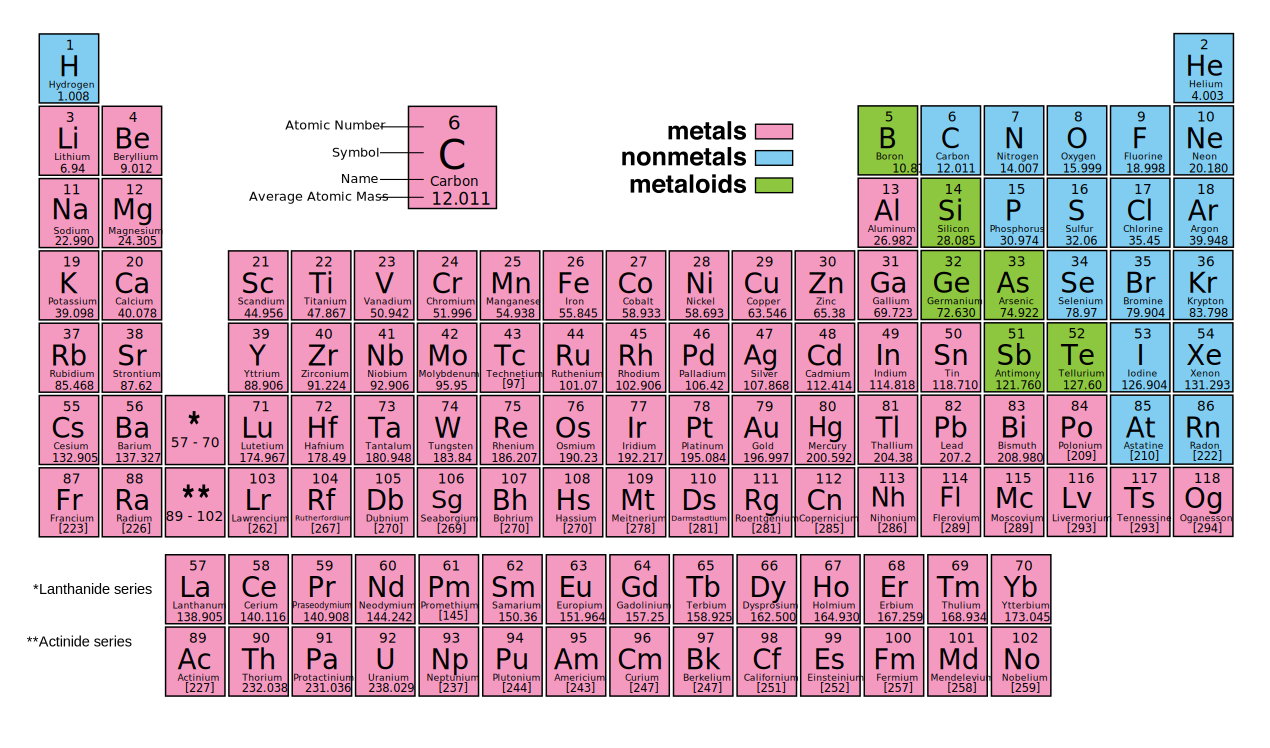
\includegraphics[width=0.7\textwidth]{../img/pte.png}
\end{center}
\end{frame}
\begin{frame}[label={sec:org9f7c494}]{Algunos apuntes de la TP que debe conocer:}
\begin{center}
\begin{tabular}{lll}
 & Nombre & Bloque\\
\hline
IA & Metales Alcalinos & s\\
IIA & M. Alcalinos Térreos & s\\
IIIA & Boroídeos & p\\
IVA & Carbonoides & p\\
VA & Calcógenos & p\\
VIA & Anfígenos & p\\
VIIA & Halógenos & p\\
0 & Gases nobles & p\\
Grupos B & Transición & d\\
Grupos A & Representativos & sp\\
Lantánidos y actínidos & Transición interna & f\\
\end{tabular}
\end{center}
\end{frame}
\begin{frame}[label={sec:orga98b78f}]{¿Qué propiedades de los elementos varían a lo largo y ancho de la Tabla periódica?}
\begin{columns}
\begin{column}{0.5\columnwidth}
\footnotesize
\begin{itemize}[<+->]
\item Existen muchas propiedades que varían a lo largo y ancho de la TP, a esas propiedades se les conoce como \emph{Propiedades periódicas}.
\item En este curso solamente estudiaremos la \emph{Electronegatividad}.
\item Electronegatividad: Tendencia de un elemento para atraer electrones [en un enlace].
\item Existen, principalmente, dos escalas de electronegatividad, de Mulliken y Pauli. Usaremos la escala de Pauli la cual toma valores desde: 0,7 a 4 (sin unidades)
\end{itemize}
\end{column}
\begin{column}{0.5\columnwidth}
\begin{figure}[htbp]
\centering
\includegraphics[width=\textwidth]{../img/en.jpeg}
\caption{Variación en aumento de la EN a lo largo y ancho de la TP}
\end{figure}
\end{column}
\end{columns}
\end{frame}
\begin{frame}[label={sec:org7802e0d}]{Configuración electrónica y TP}
\begin{itemize}
\item Habrá notado que si el elemento posee muchos electrones la configuración electrónica puede tornarse muy larga de escribir, ejemplo:
\item \ce{_38Sr} = 1s²2s²2p⁶3s²3p⁶4s²3d\textsuperscript{10}4p⁶5s²
\item En química, los electrones que participan en las reacciones químicas son los del \emph{último nivel}, dichos electrones reciben el nombre de \alert{electrones de valencia} (ev), mientras que los \guillemotleft{}otros\guillemotright{} corresponden al \guillemotleft{}kernel\guillemotright{}.
\item Es por ello que para escribir CE que resalten solo a los ev utilizamos el gas noble anterior más próximo para resumir el \guillemotleft{}kernel\guillemotright{} con ello la configuración anterior quedará:
\item \ce{_38Sr} = [Kr]5s²
\end{itemize}
\end{frame}

\section{Enlace Químico}

\begin{frame}{¿Qué es un enlace?}

	\begin{columns}
		\begin{column}{.5\textwidth}
			\begin{itemize}[<+->]
				\item Un enlace se define como la unión de dos átomos (o grupo) que conlleva a la formación de una entidad molecular independiente y estable. \cite{IUPAC2025}
				\item Revisaremos 3 tipos de enlace
				      \begin{itemize}[<+->]
					      \item Metálico
					      \item Iónico
					      \item Covalente
				      \end{itemize}
			\end{itemize}
		\end{column}

		\begin{column}{.5\textwidth}
			\begin{figure}[ht]
				\centering
				\includegraphics<1-2>[width=\textwidth]{../img/bond.jpeg}
				\only<1-2>{\caption{Imágen del benceno utilizando Microscopía de fuerza atómica}}
				\includegraphics<3>[width=\textwidth]{../img/metal.jpg}
				\only<3>{\caption{Vigas metálicas}}
				\includegraphics<4>[width=\textwidth]{../img/sal.jpeg}
				\only<4>{\caption{Sal (cristal de halita)}}
				\includegraphics<5>[width=\textwidth]{../img/coal.jpeg}
				\only<5>{\caption{Carbón}}
			\end{figure}
		\end{column}
	\end{columns}
\end{frame}

\begin{frame}{Enlace metálico}
	\begin{columns}
		\begin{column}{.5\textwidth}
			\begin{itemize}[<+->]
				\item El enlace metálico se da porque los electrones ceden sus electrones de valencia a todos los elementos del conjunto.
				\item Esta deslocalización de los electrones de debe a: la baja electronegatividad
			\end{itemize}
		\end{column}

		\begin{column}{.5\textwidth}
			\begin{figure}[ht]
				\centering
				\includegraphics[width=\textwidth]{../img/sea-electron.png}
				\caption{Teoría del \textit{Mar de electrones}}
			\end{figure}

		\end{column}
	\end{columns}

\end{frame}

\begin{frame}{Enlace Iónico}
	\begin{columns}
		\begin{column}{.5\textwidth}
			\begin{itemize}[<+->]
				\item El enlace iónico se da entre un elemento metálico y otro no-metálico.
				\item Una determinación más cuantitativas es si $\Delta EN > 1,7 $
				\item Una característica que aquí existe una cesión de electrones del metal al no-metal.
				\item De esta forma dejando al metal como \textit{catión} y al no-metal como \textit{anión}.
				\item La transferencia de electrones se da en la medida que ambos elementos queden con una \textbf{capa llena}.
			\end{itemize}
		\end{column}

		\begin{column}{.5\textwidth}
			\begin{figure}[ht]
				\centering
				\includegraphics[width=\textwidth]{../img/ionico.jpg}
				\caption{Explicación de la formación del LiF}
			\end{figure}

		\end{column}
	\end{columns}
\end{frame}

\begin{frame}{Enlace Covalente}
	\begin{columns}
		\begin{column}{.5\textwidth}
			\begin{itemize}[<+->]
				\item El enlace covalante se entre la unión de dos no-metales.
				\item En este tipo de enlaces se dice que ocurren cuando $\Delta EN < 1,7 $
				\item Dado que la diferencia de EN es pequeña, ambos elementos compiten por los electrones del otro.
				\item Existen dos tipos de enlace covalente:
				      \begin{itemize}[<+->]
					      \item Si $\Delta EN = 0$, entonces sera un enlace covalente \textbf{apolar}.
					      \item En caso contrario será un enlace covalente \textbf{polar}.
				      \end{itemize}
			\end{itemize}
		\end{column}

		\begin{column}{.5\textwidth}
			\begin{figure}[ht]
				\centering
				\includegraphics[width=\textwidth]{../img/cl2.png}
			\end{figure}

		\end{column}
	\end{columns}

\end{frame}

\begin{frame}{Estructuras de Lewis}
	\begin{columns}
		\begin{column}{.5\textwidth}
			\begin{itemize}[<+->]
				\item El nombre de Estructuras de Lewis deben el nombre a Gilber N. Lewis
				\item Científico de EEUU que en 1916 formula la \textit{regla del octeto}.
				\item Lewis desarrollo toda su teoría aún sin conocer todo el desarrollo mecanocuántico que explica en el enlace químico y, aún así usamos sus ideas hasta el día de hoy.
			\end{itemize}
		\end{column}

		\begin{column}{.5\textwidth}
			\begin{figure}[ht]
				\centering
				\includegraphics[height=0.6\textheight]{../img/lewis}
				\caption{Gilber N. Lewis 1875 - 1946}
			\end{figure}

		\end{column}
	\end{columns}

\end{frame}

\begin{frame}{Simbolos de Lewis}
	\begin{columns}
		\begin{column}{.5\textwidth}
			\begin{itemize}[<+->]
				\item Primero que todo: \textbf{solo trabajaremos con elementos representativos}
				\item Para construir una estructura de Lewis, primero se dibujarán los \textit{símbolos de lewis}.
				\item Para dibujar un símbolo de lewis bastará con rodear al elemento en sus cuatro costados con tantos puntos como electrones de valencia tenga: ejemplo Cl, Grupo VIIA = 7 e^- de valencia.
			\end{itemize}
		\end{column}

		\begin{column}{.5\textwidth}
		  \Huge
			\centering
			\only<3>{
				\Charge{0=\.}{Cl}
			}
			\only<4>{
				\Charge{0=\., 90=\.}{Cl}
			}
			\only<5>{
				\Charge{0=\., 90=\., 180=\.}{Cl}
			}
			\only<6>{
				\Charge{0=\., 90=\., 180=\., 270=\.}{Cl}
			}
			\only<7>{
				\Charge{0=\:, 90=\., 180=\., 270=\.}{Cl}
			}
			\only<8>{
				\Charge{0=\:, 90=\:, 180=\., 270=\.}{Cl}
			}
			\only<9>{
				\Charge{0=\:, 90=\:, 180=\:, 270=\.}{Cl}
			}
		\end{column}
	\end{columns}

\end{frame}

\begin{frame}{Estructuras de Lewis}
  \begin{columns}
	\begin{column}{.5\textwidth}
	  \begin{enumerate}[<+->]
	  	\item Contar los ev de todos los átomos en la molécula.
		\item Elegir el átomo central, menos electronegativo (excepto H)
		\item Dibujar enlaces del átomo central a los \textit{ligandos}.
		\item Distribuír los electrones sobrantes al átomo central y después a los \textit{ligandos}.
		  \item Todos los átomos cumplen la \textit{regla del octeto} o \textit{dueto} para el hidrógeno y se conserva el número de electrones del paso 1.
	  \end{enumerate}
	\end{column}

	\begin{column}{.5\textwidth}
	  \centering
	  \only<1>{\ce{CCl_4} = $7 \times 4 + 4 = 32$}
	  \only<2>{C = 2,55 > Cl = 3.16}
	  \only<3>{\chemfig{Cl-[7]C(-[1]Cl)(-[5]Cl)-[7]Cl}}
	  \only<4->{\chemfig{{\Charge{45=\:,135=\:,225=\:}{Cl}}-[7]C(-[1]{\Charge{45=\:,135=\:,315=\:}{Cl}})(-[5]{\Charge{135=\:,225=\:,315=\:}{Cl}})-[7]{\Charge{45=\:,315=\:,225=\:}{Cl}}}}
	\end{column}
  \end{columns}

\end{frame}

\begin{frame}{Otros tipos de enlaces}
  \begin{columns}
	\begin{column}{.5\textwidth}
	  \begin{itemize}[<+->]
\item A veces para que el átomo central o los ligandos puedan cumplir el \textit{octeto} será necesario tener más de un par de electrones en el enlace, a veces, puede ser:
  \begin{itemize}[<+->]
\item Dos pares, y se llamará \textit{enlace doble}
   \item Tres pares, u se llamará \textit{enlace triple}
   \end{itemize}
	  \end{itemize}
	\end{column}

	\begin{column}{.5\textwidth}
	  \begin{figure}[ht]
		\centering
		\only<2>{
		\chemfig{\Charge{135=\:,225=\:}{O}=C=\Charge{45=\:,315=\:}{O}}
		\caption{\ce{CO_2}}
		}
		\only<3>{
		  \chemfig{H-C~\Charge{0=\:}{N}}
		  \caption{\ce{HCN}}
		}
	  \end{figure}

	\end{column}
  \end{columns}

\end{frame}

\section{Teoría de repulsión de pares de electrones de valencia (TRPEV)}

\begin{frame}{TRPEV}
	\begin{columns}
		\begin{column}{.5\textwidth}
			\begin{itemize}[<+->]
				\item La estructuras de Lewis, si bien son útiles para determinar la unión de elementos y pares electronicos libres, no nos permite, directamente saber la disposición 3D de esta.
				\item En nuestro auxilio, utilizamos la ``Teoría de repulsión de pares eletronicos enlazantes'' (TRPEV).
				\item La cual como bien dice su nombre establece que los enlaces en una molécula, buscarán adoptar la mayor distancia entre ellos en un ambiente 3D.
				\item Esta teoría también se llama teoría de Gilliespie-Nyholm en honor a sus creadores en 1957.
			\end{itemize}
		\end{column}

		\begin{column}{.5\textwidth}
			\begin{figure}[ht]
				\centering
				\includegraphics[width=0.8\textwidth]{../img/gilliespie.png}
				\caption{Creadores de la TRPEV}
			\end{figure}
		\end{column}
	\end{columns}

\end{frame}

\section{Identificación de la geometría y polaridad de las moléculas en función de los átomos que la componen según la TRPEV}

\begin{frame}{¿Cómo saber la disposición 3D de una molécula?}
	\begin{columns}
		\begin{column}{.5\textwidth}
			\begin{itemize}[<+->]
				\item Afortunadamente Gilliespie y Nyholm hicieron todos los cálculos por nosotros
				\item Por tanto solamente necesitamos conocer cómo se ordenan los ligandos alrededor del átomo central para determinar su geometría (disposición 3D)
			\end{itemize}
		\end{column}
		\begin{column}{.5\textwidth}
			\begin{figure}[ht]
				\centering
				\includegraphics[width=0.7\textwidth]{../img/molview.png}
				\caption{\url{https://molview.org}}
			\end{figure}

		\end{column}
	\end{columns}

\end{frame}

\begin{frame}{Dime tu composición y te diré tu geometría}
	\begin{columns}
		\begin{column}{.5\textwidth}
			\begin{itemize}[<+->]
				\item Para determinar la geometría de la molécula primero utilizaremos el método ABE, AXE, o ALE
				\item Seguido revisaremos, con este método según la tabla TRPEV que geometría y ángulo de enlace corresponde

			\end{itemize}


		\end{column}

		\begin{column}{.5\textwidth}
			\begin{block}{Notación ALE}
				\begin{itemize}
					\item A = átomo central
					\item L = Ligando
					\item E = par electrónico libre del átomo central
				\end{itemize}
			\end{block}

		\end{column}
	\end{columns}
\end{frame}

\begin{frame}{TRPEV}

	\begin{figure}[ht]
		\centering
		\includegraphics[width=0.4\textwidth]{../img/trpev.png}
		\caption{\url{https://es.wikipedia.org/wiki/TRePEV}}
	\end{figure}
\end{frame}

\begin{frame}{Polaridad}
	\begin{columns}
		\begin{column}{.5\textwidth}
			La polaridad de una molécula dependerá de:
			\begin{itemize}[<+->]
				\item Su distribución de carga, si es homogénea, será \textit{apolar}
				\item En caso contrarío será \textit{polar}
			\end{itemize}
		\end{column}

		\begin{column}{.5\textwidth}
			\begin{figure}[ht]
				\centering
				\includegraphics<1>[width=0.6\textwidth]{../img/aceite}
				\includegraphics<2>[width=0.6\textwidth]{../img/agua}
			\end{figure}

		\end{column}
	\end{columns}

\end{frame}

\begin{frame}{Análisis de la distribución de carga}

\end{frame}

\section{Predicción del tipo de interacciones intermoleculares}

\begin{frame}{Tipos de interacciones intermoleculares}
  \begin{columns}
    \begin{column}{.5\textwidth}
 	\begin{itemize}[<+->]
		\item ion-ion
		\item ion-diper
     \item Fuerzas de Van der Waals
     \begin{itemize}
		\item diper-diper
		\item diper-dipin
		\item Fuerzas de dispersión (London)
	\end{itemize}
     \end{itemize}
     \end{column}
     \begin{column}{.5\textwidth}
     \end{column}
   \end{columns}
\end{frame}

\begin{frame}{Esto, cómo afecta la formación de las disoluciones en:}
  \begin{itemize}[<+->]
	\item la formación de soluciones
	\item Propiedades físicas.
	 \begin{itemize}[<+->]
	\item Solubilidad
	\item Punto de fusión
	\item Conductividad eléctrica.
	 \end{itemize}
  \end{itemize}
\end{frame}

\section{Interacciones Intermoleculares y formación de disoluciones}

\begin{frame}{¿Cómo ocurre la disolución?}
	\begin{columns}
		\begin{column}{.5\textwidth}
			\begin{itemize}[<+->]
				\item Proceso de solvatación
				\item Fuerzas soluto-solvente vs. fuerzas intramoleculares
				\item Ejemplo: NaCl en agua
			\end{itemize}
		\end{column}

		\begin{column}{.5\textwidth}
			\begin{figure}[ht]
				\centering
				\includegraphics[width=\textwidth]{../img/water-salt.jpg}
				\caption{Representación de NaCl disolviéndose en agua (esferas de \ce{Na+} y \ce{Cl-} rodeadas por \ce{H2O})}
			\end{figure}
		\end{column}
	\end{columns}
\end{frame}

\begin{frame}{Lo semejante disuele lo semejante}
	\begin{columns}
		\begin{column}{.5\textwidth}
			\begin{itemize}[<+->]
				\item Disolución de sustancias polares en solventes polares
				\item Disolución de sustancias apolares en solventes apolares
				\item Ejemplo: NaCl en agua vs. aceite en gasolina
			\end{itemize}
		\end{column}
		\begin{column}{.5\textwidth}
			\begin{figure}[ht]
				\centering
				\includegraphics[width=0.8\textwidth]{../img/vitc-sol.jpg}
				\caption{Comparación de solubilidad de la Vitamina C en diferentes solventes (menos RA más soluble) \cite{Aristizabal2016}}
			\end{figure}
		\end{column}
	\end{columns}
\end{frame}

\begin{frame}{Factores que afectan la solubilidad}
	\begin{columns}
		\begin{column}{.5\textwidth}
			\begin{itemize}[<+->]
				\item Naturaleza del soluto y solvente
				\item Temperatura:
				      \begin{itemize}
					      \item Aumento en solubilidad de sólidos en líquidos
					      \item Disminución en solubilidad de gases en líquidos
				      \end{itemize}
				\item Presión (Ley de Henry)
			\end{itemize}
		\end{column}

		\begin{column}{.5\textwidth}
			\begin{figure}[ht]
				\centering
				\includegraphics<2-4>[width=0.6\textwidth]{../img/temp-solv.jpeg}
				\includegraphics<5>[width=0.8\textwidth]{../img/henry-law.png}
				\only<2-4>{\caption{Disolver azúcar: agua fría vs caliente}}
				\only<5>{\caption{Proceso de abrir una geaseosa}}
			\end{figure}
		\end{column}
	\end{columns}

\end{frame}

\section{Influencia de las interacciones en las propiedades físicas}

\begin{frame}{Punto de fusión y ebullición}
	\begin{columns}
		\begin{column}{.5\textwidth}
			\begin{itemize}[<+->]
				\item Relación con la fuerza de las interacciones intermoleculares
				\item Comparación entre sustancias con distintos tipos de fuerza
				\item Ejemplo: agua vs. etanol vs. butano
			\end{itemize}
		\end{column}

		\begin{column}{.5\textwidth}
			\begin{figure}[ht]
				\centering
				\only<1-2>{
					\begin{tabular}{|l|l|}
						\hline
						Sustancia & \ce{T_{eb}} °C \\
						\hline
						Agua      & 100            \\
						\hline
						Etanol    & 78             \\
						\hline
						Sal       & 1465           \\
						\hline
					\end{tabular}
					\caption{Temperatura de ebullición de diferentes sustancias}
					\includegraphics<3>[width=\textwidth]{../img/ff-inter.png}
				}

			\end{figure}

		\end{column}
	\end{columns}
\end{frame}

\begin{frame}{Solubilidad en diferentes solventes}
	\begin{columns}
		\begin{column}{.5\textwidth}
			\begin{itemize}[<+->]
				\item Diferencias en solubilidad según el tipo de interacción
				\item Ejemplo: NaCl soluble en agua pero insoluble en hexano
				\item Importancia en la industria farmacéutica
			\end{itemize}
		\end{column}

		\begin{column}{.5\textwidth}
			\begin{table}[ht]
				\centering
				\begin{tabular}{|l|l|}
					\hline
					Sustancia  & Solubilidad \\
					\hline
					NaCl       & 36          \\
					\hline
					KCl        & 34          \\
					\hline
					\ce{NaNO3} & 88          \\
					\hline
					Azúcar     & 203         \\
					\hline
				\end{tabular}
				\caption{Tabla de solubilidad cada 100g de agua a 20°C}
			\end{table}
		\end{column}
	\end{columns}
\end{frame}

\begin{frame}{Conductividad eléctrica en soluciones}
	\begin{columns}
		\begin{column}{.5\textwidth}
			\begin{itemize}[<+->]
				\item Diferencia entre solutos iónicos y covalentes.
				\item Ejemplo: NaCl en agua vs. azúcar en agua.
				\item Importancia en electrolitos biológicos.
			\end{itemize}
		\end{column}

		\begin{column}{.5\textwidth}
			\begin{figure}[ht]
				\centering
				\includegraphics<1-2>[width=\textwidth]{../img/disolucion.png}
				\only<1-2>{\caption{Representación iones en disolución}}
				\includegraphics<3>[width=\textwidth]{../img/electrolito-no-ele.jpg}
				\only<3>{\caption{Electrolito vs No electrolitos}}
			\end{figure}
		\end{column}
	\end{columns}
\end{frame}

\section{Relación entre estructura y funcionalidad en sustancias cotidianas}

\begin{frame}{Aplicaciones en la vida diaria}
	\begin{columns}
		\begin{column}{.5\textwidth}
			\begin{itemize}[<+->]
				\item ¿Por qué los aceites no se mezclan con el agua?
				\item ¿Por qué el alcohol se evapora rápido?
				\item ¿Por qué el hielo flota en agua?
			\end{itemize}
		\end{column}
		\begin{column}{.5\textwidth}
			\begin{figure}[ht]
				\centering
				\includegraphics<1>[width=\textwidth]{../img/inmiscible.jpeg}
				\includegraphics<2>[width=\textwidth]{../img/boiling-points.png}
				\includegraphics<3>[width=\textwidth]{../img/water-ice.jpg}
			\end{figure}
		\end{column}
	\end{columns}
\end{frame}

\begin{frame}{Materiales y tecnología}
	\begin{columns}
		\begin{column}{.5\textwidth}
			\begin{itemize}[<+->]
				\item Polímeros hidrofóbicos en ropa impermeable
				\item Solubilidad en medicamentos
				\item Electrólitos en baterías
			\end{itemize}
		\end{column}
		\begin{column}{.5\textwidth}
			\begin{figure}[ht]
				\centering
				\includegraphics<1>[width=0.8\textwidth]{../img/hidrophobic.jpeg}
				\includegraphics<2>[width=0.8\textwidth]{../img/drug-transport.png}
				\includegraphics<3>[width=0.6\textwidth]{../img/battery-flow.jpeg}
			\end{figure}
		\end{column}
	\end{columns}
\end{frame}

\section{Cierre y Reflexión}

\begin{frame}{Resumen general}
	\begin{itemize}[<+->]
		\item Tipos de interacciones intermoleculares
		\item Influencia en solubilidad y propiedades físicas
		\item Aplicaciones en la vida cotidiana
	\end{itemize}
\end{frame}

\begin{frame}{Preguntas y discusión}
	\begin{columns}
		\begin{column}{.5\textwidth}
			\begin{itemize}[<+->]
				\item Espacio para resolver dudas
				\item Pregunta final: ¿Cómo podrías aplicar estos conceptos en tu campo de estudio o en tu vida diaria?
			\end{itemize}
		\end{column}

		\begin{column}{.5\textwidth}
			\begin{figure}[ht]
				\centering
				\includegraphics[width=0.8\textwidth]{../img/discussion.jpg}
			\end{figure}

		\end{column}
	\end{columns}

\end{frame}

\begin{frame}[allowframebreaks]{Bibliografía}
	\begin{thebibliography}{Scerri, 2007}
		\footnotesize
		\setbeamertemplate{bibliography item}[book]
		\bibitem[Chang, 2011]{Chang2011}
		Chang, Raymond
		\newblock \emph{Fundamentos de Química}
		\newblock McGraw Hill, 2011

		\setbeamertemplate{bibliography item}[book]
		\bibitem[Chang, 2010]{Chang2010}
		Chang, Raymond
		\newblock \emph{Química}, 10° Edición
		\newblock McGraw Hill, 2010

		\setbeamertemplate{bibliography item}[book]
		\bibitem[Brown, 2009]{Brown2009}
		Brown, T.L; LeMay, H.E; Bursten, B.E y col.
		\newblock \emph{Química: La Ciencia Central}
		\newblock Pearson, 2009

		\setbeamertemplate{bibliography item}[book]
		\bibitem[Petrucci, 2011]{Petrucci2010}
		Petrucci, R.H; Herring, F.G; Madura, J.D y Bissonnette, C.
		\newblock \emph{Química General: Principios y Aplicaciones Modernas} 10° Edición
		\newblock Pearson, 2011

		\setbeamertemplate{bibliography item}[book]
		\bibitem[Serway, 2008]{Serway2008}
		Serway, R. y Jewett, J.
		\newblock \emph{Física para Ciencias e Ingeniería}, 7° Edición
		\newblock Brooks/Cole, 2008

		\setbeamertemplate{bibliography item}[online]
		\bibitem[Labnews, 2019]{Labnews2019}
		Laboratory news
		\newblock \emph{Alternative periodic tables}
		\newblock \url{https://www.labnews.co.uk/article/2029799/alternative-periodic-tables}

		\setbeamertemplate{bibliography item}[online]
		\bibitem[Lifeder, 2022]{Lifeder2022}
		Lifeder
		\newblock \emph{Tríadas de Döbereiner}
		\newblock \url{https://www.lifeder.com/triadas-de-dobereiner/}

		\setbeamertemplate{bibliography item}[online]
		\bibitem[Energía Nuclear, 2023]{Nuclear2023}
		Energía Nuclear
		\newblock \emph{Ley de las Octavas de Newlands}
		\newblock \url{https://energia-nuclear.net/quimica/tabla-periodica/linea-del-tiempo/ley-de-las-octavas}

		\setbeamertemplate{bibliography item}[book]
		\bibitem[Scerri, 2007]{Scerri2007}
		Scerri, Eric.
		\newblock \emph{The Periodic Table: It's Story and Its Significance}
		\newblock Oxford University Press, 2007

		\setbeamertemplate{bibliography item}[article]
		\bibitem[Aristizabal, 2016]{Aristizabal2016}
		Dyna
		\newblock \emph{Determinación numérica de la solubilidad de la vitamina C en diferentes solventes, para la extracción selectiva o para la incorporación en formulaciones orientadas al cuidado, bienestar y salud de la piel}
		\newblock \url{https://doi.org/10.15446/dyna.v83n199.54828}

		\setbeamertemplate{bibliography item}[online]
		\bibitem[IUPAC, 2025]{IUPAC2025}
		International Union of Pure and Applied Chemistry
		\newblock \emph{IUPAC Compendium of Chemical Terminology, 5th ed.}
		\newblock \url{https://doi.org/10.1351/goldbook.CT07009}

	\end{thebibliography}
\end{frame}

\end{document}
